% \documentclass[nobib]{tufte-book}
\documentclass[
	a4paper, % Paper size, use either a4paper or letterpaper
	10pt, % Default font size, can also use 11pt or 12pt, although this is not recommended
	% unnumberedsections, % Comment to enable section numbering
	twoside, % Two side traditional mode where headers and footers change between odd and even pages, comment this option to make them fixed
]{LTJournalArticle}

% \usepackage{amsmath}
% \usepackage{graphicx}
\usepackage{hyperref}

% \usepackage[style=verbose, autocite=footnote, backend=biber]{biblatex}
% \usepackage{biblatex}
\addbibresource{references.bib}

\runninghead{Decent Cloud: A Decentralized Cloud That You Can Trust}

\title{Decent Cloud: A Decentralized Cloud Platform That You and Your Business Can Trust} % Article title, use manual lines breaks (\\) to beautify the layout

\author{%
	Anonymous
}


% Full-width abstract
\renewcommand{\maketitlehookd}{%
	\begin{abstract}
        This paper introduces a novel decentralized cloud platform that bridges the gap between traditional centralized cloud services and fully decentralized systems. Our platform enables developers to access tailored virtual or physical servers, offered by identifiable node providers with established reputations and backed by robust legal contracts.

Unlike typical decentralized platforms, our approach requires node providers to build long-term reputations, allowing users to select providers based on their reliability and performance. This reputation-based system addresses key challenges in both centralized and existing decentralized cloud models, including vendor lock-in, opaque pricing, and barriers to entry.

In addition to the regular servers, our platform also supports sensitive data processing through Confidential Computing VMs and facilitates GPU node rental for ML and AI applications at competitive rates. By running the control plane on a blockchain while keeping the performance-sensitive data plane on the regular Internet, we overcome limitations of conventional web3 platforms, allowing seamless integration of legacy applications.

Decent Cloud offers substantial benefits for both node providers and developers. {\bf Developers} can (a) find cloud providers suitable for their specific needs, (b) obtain legal guarantees and SLA agreements typically expected by businesses, and (c) utilize services from multiple providers (multi-cloud deployments) with minimal added complexity. For {\bf Node Providers}, it provides access to the trillion-dollar crypto market and this way reach a vast global user base. Crucially for node providers, Decent Cloud mitigates the "race to the bottom" pricing that plagues other decentralized cloud computing platforms, by implementing transparent, decentralized pricing {\em and} a reputation system that encourages and rewards honest behavior.

	\end{abstract}
}

\begin{document}

\maketitle

% \frontmatter

% \tableofcontents

% \mainmatter

\section{Introduction}
\label{sec:introduction}

Cloud computing has revolutionized data storage and processing, offering on-demand access to vast computational resources without direct user management. However, the current landscape is dominated by a few major providers, leading to concerns about vendor lock-in, security vulnerabilities, and resource inefficiencies.

This paper presents a novel decentralized cloud platform that addresses these challenges while leveraging the strengths of both centralized and decentralized models. Our approach combines the reliability and performance of traditional cloud services with the flexibility and democratization of decentralized systems, creating a more robust, efficient, and user-centric cloud computing ecosystem.
\subsection{Background and Motivation}
\label{sec:background}

In response to these challenges, decentralized cloud computing has emerged as a promising alternative. This approach distributes data and processes across multiple machines, or nodes, each equipped with its own processing power and storage. This distribution can lead to more efficient resource allocation and utilization, as resources can be dynamically shared among nodes based on demand.

Our objective is to address the inherent issues of centralized cloud computing by constructing a secure and trustworthy system. This is achieved through the implementation of robust security measures and a reputation system, which collectively enhance the reliability and integrity of the platform.

Furthermore, we aim to promote transparency and democratic principles within the system by employing a decentralized matching engine and a Decentralized Autonomous Organization (DAO) model for governance. This approach is intended to stimulate competition and innovation in the field.

By lowering the barriers to becoming a cloud provider and offering a global rating system for all cloud providers, we enable developers to select providers based on their specific needs and preferences. This approach not only fosters a more competitive and innovative environment but also empowers developers by providing them with more choice and control over their cloud computing solutions.

\subsection{Academic research}

Decentralized cloud computing has garnered significant attention in the academic community as a viable alternative to centralized cloud models. Research in this domain explores various approaches to enhancing the efficiency, security, and scalability of cloud services through decentralization.

Xu Chen's work on "Decentralized Computation Offloading Game for Mobile Cloud Computing" \cite{chen2014decentralized} proposes a game-theoretic framework for efficient computation offloading in mobile cloud environments. This work highlights the potential of decentralized models in optimizing resource allocation, particularly in scenarios involving mobile devices with limited computational capabilities.
Similarly, Sladana Jošilo and G. Dán in their paper "Selfish Decentralized Computation Offloading for Mobile Cloud Computing in Dense Wireless Networks" \cite{josilo2018selfish} investigate the dynamics of decentralized computation offloading in dense wireless networks. Their research underscores the challenges of coordinating decentralized nodes and the importance of incentive mechanisms in ensuring efficient resource sharing.

Kunal et al.~\cite{kunal2019overview} explore fog computing as a decentralized layer between users and cloud servers, aiming to reduce latency and enhance service delivery. This research aligns with the broader goal of decentralization by distributing computational tasks closer to the edge, thereby improving responsiveness and reducing the load on central servers.

Nguyen et al.~\cite{nguyen2020integration} provide a comprehensive review of integrating blockchain with Cloud of Things (CoT), emphasizing the potential of blockchain to address decentralization challenges, enhance data privacy, and secure network transactions. Their work provides insights into the benefits of combining blockchain technology with decentralized cloud architectures.

Wenjuan Li et al. proposed a blockchain-based trust management system in cloud computing \cite{li2021blockchain}, which aligns closely with our platform's reputation-based approach. Their research illustrates how blockchain can be leveraged to establish trust among decentralized nodes, ensuring reliable and secure service delivery.

Chegini et al.~\cite{chegini2021process} discuss the automation of tasks and processes in the IoT-Fog-Cloud ecosystem, addressing big data and heterogeneity challenges. Their work highlights the need for decentralized solutions to manage the complexity and scale of modern cloud environments effectively.

Finally, Espinel Sarmiento et al.~\cite{sarmiento2021decentralized} survey the application of Software Defined Networks (SDN) in managing distributed Cloud-Edge infrastructures. This research is particularly relevant to our platform, as it demonstrates how SDN can facilitate the coordination and management of decentralized resources across a distributed cloud environment.

\subsection{Industry projects}

In recent years, several industry projects have attempted to build decentralized cloud platforms. These platforms leverage blockchain technology to create a network of independent node providers that can store data or run arbitrary workloads in a decentralized fashion, and highly resilient to malicious actors.

\begin{itemize}
    \item {\bf Filecoin} (\url{https://filecoin.io/}): Filecoin is a decentralized storage network designed to store and retrieve data in a distributed fashion. By incentivizing storage providers through its native cryptocurrency, Filecoin creates a competitive marketplace for data storage. While Filecoin excels in decentralized storage, it does not extend to compute resources. In contrast, our platform aims to integrate both storage and compute capabilities, offering a more holistic cloud solution.

    \item {\bf Storj} (\url{https://www.storj.io/}): Storj is a decentralized cloud storage platform that focuses on secure and distributed data storage. It fragments and encrypts data before distributing it across its network, ensuring high levels of security and redundancy. Similar to Filecoin, Storj is storage-centric and does not offer compute resources. Our platform distinguishes itself by providing a marketplace that includes both storage and compute services.

    \item {\bf Sia} (\url{https://sia.tech/}): Sia operates as a decentralized storage platform that leverages global hard drive capacity to create a distributed data storage network. While Sia effectively reduces storage costs and enhances data redundancy, it lacks the ability to offer compute resources. Additionally, it does not incorporate a reputation-based system for node providers. Our platform addresses these gaps by integrating compute capabilities and establishing a reputation system to enhance trust and reliability.

    \item {\bf Arweave} (\url{https://www.arweave.org/}): Arweave offers a unique approach to data storage by providing permanent and sustainable storage solutions. It is particularly suited for archiving and storing immutable data. However, Arweave's focus on storage limits its applicability in scenarios requiring compute resources. Our platform expands on this by supporting both storage and compute, catering to a broader range of cloud computing needs.

    \item {\bf DFINITY} (\url{https://dfinity.org/}): DFINITY's Internet Computer represents a significant step toward decentralized cloud computing by enabling developers to host entire applications on its decentralized network. Despite its innovation, the Internet Computer's reliance on the Consensus protocol imposes performance limitations, particularly for high-throughput applications. Our platform, by contrast, separates the control and data planes, allowing for higher performance and broader applicability across diverse workloads.

    \item {\bf Akash Network} (\url{https://akash.network/}): Akash Network is a decentralized cloud computing platform that focuses on offering compute resources through a permissionless marketplace. Akash allows users to rent computing power from providers across the globe, targeting workloads such as web hosting, machine learning, and containerized applications. While Akash shares similarities with our platform, our solution emphasizes a more comprehensive approach, integrating robust reputation systems and legal frameworks to ensure quality and reliability, which many users see as essential.

    \item {\bf Golem} (\url{https://golem.network/}): Golem functions as a decentralized supercomputer that aggregates the computational power of user machines worldwide. It is particularly well-suited for compute-intensive tasks such as rendering and scientific simulations. However, Golem's focus on specialized compute tasks limits its versatility as a general-purpose cloud platform. Our platform aims to provide a more flexible solution that accommodates a wide range of workloads, from basic web hosting to complex AI processing.

    \item {\bf iExec} (\url{https://iex.ec/}): iExec provides a decentralized marketplace for cloud computing resources, primarily serving decentralized applications (DApps) on blockchain networks. While iExec offers an efficient solution for DApp developers, its reliance on the Consensus protocol can slow down execution times, limiting its use for performance-sensitive applications. Our platform, by contrast, is designed to serve a broader spectrum of applications, with a focus on minimizing latency and maximizing performance.

    \item {\bf Aethir} (\url{https://www.myedge.io/}): Aethir offers a decentralized marketplace for renting GPU resources, specifically targeting machine learning (ML) and artificial intelligence (AI) workloads. By focusing on GPU availability, Aethir addresses a critical need in the AI and ML communities. Our platform incorporates similar GPU rental capabilities but extends the offering to include other compute and storage resources, providing a more comprehensive cloud solution.

    \item {\bf Cudos} (\url{https://www.cudos.org/}): Cudos is a decentralized cloud computing platform that aims to bridge the gap between cloud and blockchain by providing compute resources for blockchain and non-blockchain applications. Cudos supports a wide range of workloads, from simple hosting to complex decentralized finance (DeFi) applications. Our platform builds on these ideas by offering an even more integrated approach, combining compute, storage, and reputation systems within a single ecosystem.

    \item {\bf ICN (Impossible Cloud Network)} (\url{https://icn.global/}): The Impossible Cloud Network (ICN) is a decentralized approach to cloud infrastructure, providing a platform for managing hardware and cloud resources. It leverages decentralized technologies to ensure data security, integrity, and resiliency. ICN's approach to managing global cloud resources aligns with our platform's goal of mitigating vendor lock-in while enhancing transparency and control. Our platform further differentiates itself by integrating a reputation system and legal frameworks to ensure service quality and compliance.

    \item {\bf Fluence} (\url{https://fluence.dev/}): Fluence offers a decentralized serverless platform that enables developers to deploy applications without the need for centralized servers. It provides a peer-to-peer network for executing code, using a special-purpose language called Aqua for cryptographic proofs. While Fluence's approach is innovative, the need for specialized language limits its flexibility. Our platform, in contrast, supports a broader range of programming languages and environments, and integrates a reputation system to ensure service quality and compliance, making it accessible to a wider audience and a wider range of use cases.
\end{itemize}

These works highlight the growing interest in decentralized cloud computing and the potential benefits it can offer.
However, despite these efforts there is still a need for a comprehensive solution that addresses the issues of the current cloud computing paradigm while leveraging the benefits of decentralization. This is the problem that our proposed decentralized cloud platform aims to solve and in the following sections we provide an outline of how we plan to do this.

\begin{figure*}[ht]
    \centering
    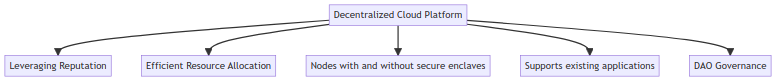
\includegraphics[width=\textwidth]{figures/proposed-solution.png}
    \caption{An illustration of the proposed solution.}
\end{figure*}

\section{Problem Statement}
\label{sec:problem_statement}

The current cloud computing landscape is dominated by a handful of large providers, including Amazon Web Services (AWS), Google Cloud Platform (GCP), and Microsoft Azure, which together control roughly 70\% of the cloud computing market, as of 2024. While these providers offer a comprehensive range of services spanning basic compute and storage to advanced machine learning and analytics tools, this centralized model presents several significant challenges:

\begin{itemize}
    \item \textbf{Vendor lock-in:} The choice of a cloud provider often becomes a long-term commitment due to:
    \begin{itemize}
        \item Proprietary APIs and services that are not easily portable
        \item Substantial costs and technical challenges associated with migrating data and applications
        \item Pricing models that incentivize increased usage within a single ecosystem
    \end{itemize}

    \item \textbf{Limited control and transparency:} Users face significant constraints in managing their cloud resources:
    \begin{itemize}
        \item Lack of granular control over data storage locations and processing methods
        \item Limited visibility into the underlying infrastructure and its performance characteristics
        \item Difficulty in optimizing applications due to the abstracted nature of cloud services
    \end{itemize}

    \item \textbf{Data privacy and security concerns:} Centralized cloud providers present attractive targets for cyberattacks:
    \begin{itemize}
        \item A single breach can potentially compromise vast amounts of data across multiple clients
        \item Users must trust the provider's security measures without full transparency
        \item Compliance with varying international data protection regulations becomes complex
    \end{itemize}

    \item \textbf{Cost and resource inefficiencies:} The pricing structures of major cloud providers can lead to financial inefficiencies:
    \begin{itemize}
        \item Complex, often opaque pricing models make cost prediction and management challenging
        \item Users frequently over-provision resources to ensure performance, leading to waste
        \item Lack of a true pay-per-use model for many services results in unnecessary expenses
    \end{itemize}
\end{itemize}

These issues have varying impacts across different stakeholders in the cloud computing ecosystem:

\begin{itemize}
    \item \textbf{Individual Developers:} Face barriers to experimentation and innovation due to high costs and complex management of cloud resources. They may struggle to scale their projects efficiently as requirements grow.

    \item \textbf{Startups:} Often find themselves locked into a specific provider early in their development, limiting future flexibility. They may face sudden cost increases as they scale, impacting their financial planning and viability.

    \item \textbf{Enterprises:} Struggle with vendor lock-in, which can impact long-term strategic decisions. They face significant challenges in maintaining regulatory compliance across different regions and in protecting sensitive data.

    \item \textbf{Government and Non-Profit Organizations:} May face difficulties in ensuring data sovereignty and meeting strict security requirements. Budget constraints can limit their ability to leverage advanced cloud services effectively.
\end{itemize}

Addressing these challenges is crucial for fostering a more open, efficient, and innovative cloud computing ecosystem. The need for a solution that provides greater flexibility, transparency, and cost-effectiveness while maintaining robust security and performance is evident across all sectors of the industry.

\section{Proposed Solution}
\label{sec:proposed_solution}

To address the limitations of the current centralized cloud computing model, we propose a novel decentralized cloud platform that combines the best aspects of traditional cloud services with the advantages of decentralized systems. Our solution is designed to tackle each of the key issues identified in the problem statement while introducing innovative features that enhance flexibility, security, and efficiency.

\subsection{Core Components of the Solution}

\subsubsection{Decentralized Infrastructure}
Our platform leverages a network of independent node providers, each capable of hosting and executing arbitrary workloads. This approach:
\begin{itemize}
    \item Mitigates vendor lock-in by offering a diverse ecosystem of providers
    \item Enhances resilience by distributing resources across nodes of different providers
    \item Improves resource utilization by tapping into underused computational capacity
\end{itemize}

\subsubsection{Reputation-Based Trust System}
\label{subsec:reputation_system}

Unlike typical Web3 solutions that rely on consensus mechanisms to mitigate the Byzantine Fault Tolerance (BFT) problem --- allowing up to 50\% (or a bit less on some platforms) of the network to be malicious --- our platform takes a different approach. We primarily rely on conventional legal contracts and Service Level Agreements (SLAs), supplemented by a robust blockchain-tracked reputation system. This dual approach ensures accountability through traditional means while providing an additional layer of trust and transparency.

In the anonymous blockchain space, an actor is more likely to behave maliciously than in the real world. In the real world there is a lot more at stake than in the blockchain space, an actor would be much less likely to behave maliciously, given that they risk suffering both legal and financial consequences for malicious behavior. Malicious behavior may still occur, but the potential benefit of such behavior needs to clearly compensate the potential cost, which may come in the form of a loss of the long-term financial benefit and the potential financial loss in the following legal processes, as analyzed in more details in Section~\ref{sec:math_model}.

Decent Cloud is designed with this in mind, and it focuses on incentivizing honest behavior and providing  high-quality service while implementing mechanisms to penalize poor performance or malicious actions. Good reputation is hard to earn, and it's easy to lose. Especially if big clients (with high reputation) are dissatisfied with the provided services.

\paragraph{Building Reputation:}
Node providers and developers accrue reputation through successful transactions and positive interactions on the platform:

\begin{itemize}
    \item Each completed transaction between a developer and a node provider results in a 2\% transaction fee, from which there is a 1\% increase in both parties' reputation scores.
    \item Consistent user satisfaction contributes to gradual reputation increases of node providers over extended periods and numerous transactions.
    \item Developers who rent many resources or spend significant amounts over longer periods of time will have higher reputation scores than those who do not.
\end{itemize}

\paragraph{Reputation Dynamics:}
Our system introduces an innovative approach to managing reputation:

\begin{itemize}
    \item Both node providers and developers build reputation through successful transactions.
    \item Rather than complicating the platform to autonomously track and judge honest behavior, we empower users to report and penalize malicious behavior.
    \item If dissatisfied with a service or collaboration, a user can choose to reduce another party's reputation. This action comes at a cost: the sender's reputation decreases by the amount spent, while the receiver's reputation decreases by a higher amount, such as 200%.
\end{itemize}

This mechanism offers several advantages:

\begin{itemize}
    \item Robustness: It's straightforward to implement and reason about.
    \item Quality Incentive: It motivates node providers to maintain high-quality service and prioritize user satisfaction.
    \item Resilience against Malicious Actors: Malicious node providers would quickly acquire poor reputations, limiting their ability to attract new users. Similarly, malicious developers quickly lose power to hurt the reputation of others, as they lose their own reputation in the process.
\end{itemize}

\paragraph{Reputation System Impact:}

This dynamic reputation system empowers users to make informed decisions when selecting node providers. It addresses trust and security concerns associated with decentralized systems while preserving the performance advantages of traditional cloud services. All reputation scores are publicly visible and immutably recorded on the blockchain, ensuring transparency and creating a reliable history of interactions and service quality.

\subsubsection{Efficient Resource Allocation}

Our platform can be used to ensure optimal resource allocation. For instance:
\begin{itemize}
    \item Task requirements can be matched with available node resources in real-time
    \item Dynamic load balancing optimizes resource utilization across the network
    \item Pricing is transparent and competitive, driven by market demand
\end{itemize}

This approach allows users to tackle the cost inefficiencies and opaque pricing models of traditional centralized providers.

\subsubsection{Enhanced Security and Privacy}

The system supports sensitive data processing and storage using Confidential Computing VMs, and also facilitates the rental of GPU nodes for Machine Learning (ML) and Artificial Intelligence (AI) training and inference applications at reasonable market prices, catering to different developer preferences. Some developers may opt for the lowest cost GPUs irrespective of node provider reputation and confidentiality guarantees, while others may prefer high-end GPUs with higher node provider reputation. This flexibility accommodates all developer categories, a feature unique to this platform.

For some use cases, such as storing and rotating tokens, certificates, and other secrets, developers will need nodes with additional security. For these use cases, platform will support Confidential Containers\cite{brasser2022trusted}.

To address data privacy and security concerns, our platform offers:
\begin{itemize}
    \item Support for Confidential Computing VMs, enabling secure processing of sensitive data
    \item End-to-end encryption for data in transit and at rest
    \item Granular control over data location and processing parameters
\end{itemize}

\subsection{Addressing Specific Challenges}

\subsubsection{Overcoming Vendor Lock-in}
Our platform's open architecture and standardized interfaces allow for easy migration between providers, addressing the vendor lock-in issue prevalent in centralized systems.

\subsubsection{Improving Control and Transparency}
Users have unprecedented visibility into the underlying infrastructure and can choose specific nodes or node providers based on their requirements, enhancing control and transparency.

\subsubsection{Enhancing Cost-Effectiveness}
The platform's market-driven pricing model and efficient resource allocation system ensure that users only pay for the resources they actually use, addressing the cost inefficiencies of traditional cloud services.

\subsection{Innovative Features}

\subsubsection{Wide Range of Applications}
Our platform supports diverse applications, from scientific high-performance computing and machine learning to web hosting and data storage, catering to a broad spectrum of user needs.

\subsubsection{DAO Governance}
We implement a Decentralized Autonomous Organization (DAO) model for platform governance, ensuring transparency and community-driven decision-making.

\subsubsection{Blockchain-Based Control Plane}
By running the control plane on a blockchain, we ensure transparent and immutable record-keeping for financial transactions and reputation tracking, while keeping the performance-sensitive data plane on the regular internet for optimal speed.

\subsection{Benefits for Stakeholders}

\subsubsection{For Developers}
\begin{itemize}
    \item Access to a diverse range of computational resources
    \item Flexibility to choose providers based on specific needs
    \item Potential for significant cost savings
\end{itemize}

\subsubsection{For Node Providers}
\begin{itemize}
    \item Opportunity to monetize unused computational resources
    \item Access to a global market of users
    \item Incentives for maintaining high-quality service through the reputation system
\end{itemize}

\begin{figure*}[h]
    \centering
    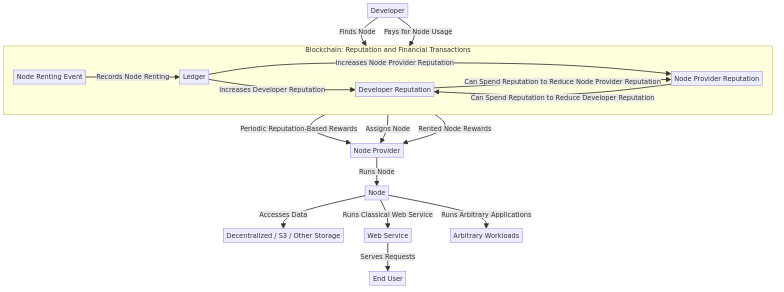
\includegraphics[width=\textwidth]{figures/proposed_architecture.png}
    \caption{Proposed platform architecture.}
    \label{fig:proposed-architecture}
\end{figure*}

Figure~\ref{fig:proposed-architecture} illustrates the architecture of our proposed platform, showcasing how these components interact to create a robust, efficient, and user-centric cloud computing ecosystem.

In the following sections, we will delve deeper into the technical details of each component, exploring how they work together to realize the full potential of decentralized cloud computing.

\section{Incentive Analysis for Malicious Behavior in Decentralized Systems}

\subsection{Introduction}

Understanding the incentives that could drive malicious behavior is crucial for enhancing the security and robustness of decentralized systems. The aim is to provide a nuanced understanding of the conditions under which malicious activities are more likely, offering insights for designing secure systems that do not need to rely on conventional consensus-based BFT schemes.

\subsection{Model Variables}

\begin{itemize}
    \item \( P(B_m), P(B_h) \) : Probability distributions for the expected benefits from malicious and honest behavior.
    \item \( P(C_m), P(C_h) \) : Probability distributions for the financial costs.
    \item \( P(R_m), P(R_h) \) : Probability distributions for the financial equivalent of reputation loss or gain, respectively for malicious and honest behavior.
    \item \( P(T_m), P(T_h) \) : Probability distributions for the time required for malicious and honest behavior.
\end{itemize}

\subsection{Model Formulation}

The expected net benefits, adjusted for time, can be modeled as:

\[
    E[N_m] = \frac{E[B_m]}{E[T_m]} - (E[C_m] + E[R_m])
\]
\[
    E[N_h] = \frac{E[B_h]}{E[T_h]} - (E[C_h] + E[R_h])
\]

Here, \( E[C_m] + E[R_m] \) and \( E[C_h] + E[R_h] \) represent the total expected costs for malicious and honest behavior, respectively. These costs include both the financial costs and the financial equivalent of reputation loss.

\subsection{Conditions for Malicious Behavior}

Malicious behavior is more likely if \( E[N_m] > E[N_h] \).

\subsection{Proof}

\textbf{Theorem:} Malicious behavior is more likely to occur if and only if \( E[N_m] > E[N_h] \).

\textbf{Proof:}

We aim to prove that malicious behavior is more likely when the expected net benefit of malicious behavior \( E[N_m] \) is greater than that of honest behavior \( E[N_h] \).

The condition \( E[N_m] > E[N_h] \) simplifies to:

\[
    \frac{E[B_m]}{E[T_m]} - (E[C_m] + E[R_m]) > \frac{E[B_h]}{E[T_h]} - (E[C_h] + E[R_h])
\]

Rearranging terms, we get:

\[
    \frac{E[B_m]}{E[T_m]} - \frac{E[B_h]}{E[T_h]} > (E[C_h] + E[R_h]) - (E[C_m] + E[R_m])
\]

This inequality shows that malicious behavior is more likely when the expected time-adjusted benefit of malicious behavior over honest behavior is greater than the expected net cost difference, which includes both the financial costs and the financial equivalent of reputation loss for both behaviors.

Therefore, malicious behavior is more likely to occur if and only if \( E[N_m] > E[N_h] \).

\textbf{Q.E.D.}

\section{Implementation}
\label{sec:implementation}

% TODO: The implementation section is detailed and informative. However, it could benefit from more visual aids, such as diagrams or flowcharts, to illustrate the relationships between different components.
% TODO: Consider adding a subsection on scalability and performance considerations, as these are crucial aspects of any cloud platform.

The proposed decentralized cloud platform consists of several key components:

\begin{itemize}
    \item \textbf{Nodes and Networking:} The platform runs numerous nodes, and each node adds its resources such as processing power, storage, and bandwidth. The network functions on a divide-and-conquer principle, minimizing communication between different applications running on the network. This strategy enables the network to scale and accommodate numerous nodes and tasks.

    \item \textbf{Reputation System:} The platform uses a blockchain-based system to ensure the security, transparency, and fairness of resource allocation. Smart contracts are utilized to verify that node providers, nodes, and developers are all acting appropriately, and that each party is suitably rewarded for their contributions or penalized for any misconduct.

    \item \textbf{Token Economics:} The platform employs a distinct dual-token system: one that can be used for transactional purposes and another for reputation tracking. The transactional token facilitates financial interactions between node providers and developers, while the reputation token, non-exchangeable in nature, is earned by node providers and developers during transactions.

    \item \textbf{Application Support:} The platform supports a wide range of applications, from scientific computing and machine learning to web hosting and data storage. The platform provides APIs and SDKs that simplify the process for developers to build and deploy their applications on the platform.
\end{itemize}


\subsection{Nodes and Networking}
\label{sec:nodes_and_networking}

The foundation of the proposed decentralized cloud platform lies in its nodes and the networking infrastructure that connects them. The platform operates on a multitude of nodes, each contributing resources such as processing power, storage, and bandwidth. This section provides a detailed overview of the nodes and networking component of the platform.

\subsubsection{Nodes}
\label{subsec:nodes}

In the context of our platform, a node is a computing device that participates in the network. Each node contributes its computational resources, including processing power (CPU), memory (RAM), storage (hard disk or SSD), and network bandwidth. Nodes can vary in size, from personal computers to large data center servers. This diversity in node capabilities is a strength of the platform, as it allows for a wide range of application requirements.

Each node operates a software client that enables its participation in the network. This client manages the node's resources, communicates with other nodes, and executes assigned tasks. The client software is designed to be lightweight and efficient, minimizing its impact on the node's performance.

\subsubsection{Networking}
\label{subsec:networking}

The networking component of the platform connects nodes and facilitates their communication. The network employs a divide-and-conquer approach, where nodes belonging to a specific developer form a smaller subnetwork or cluster. These clusters maintain direct communication within themselves, and communication between different clusters is minimal unless explicitly established by the developer.

Node providers, who typically host many Nodes or Virtual Machines (VMs), do not need to provide a public IPv4 address for each Node. This is crucial as IPv4 addresses are a scarce resource. Instead, node providers only need to port forward, thereby publicly exposing a few ports for each Node. These ports can be used for peering different nodes of the same developer. For example, some developers may peer nodes with \href{https://nats.io/}{Nats.io}, while others might use \href{https://www.wireguard.com/}{WireGuard}, but any other solution of the developer's choice would work.

Node providers also need to have HTTP and HTTPS ingress, on which a reverse proxy is set up. This reverse proxy forwards requests to the appropriate VM using Server Name Indication (SNI) technology, i.e., based on the target domain name. This routing can be done {\em without} SSL termination to prevent Node providers from being able to snoop all ingress traffic. For this, tools like \href{https://www.haproxy.com/blog/enhanced-ssl-load-balancing-with-server-name-indication-sni-tls-extension}{HAProxy} or recent versions of \href{https://nginx.org/en/docs/stream/ngx_stream_ssl_preread_module.html}{Nginx} can be used. This approach improves security, as it prevents node providers from inspecting traffic to and from nodes.

The illustrated networking approach minimizes communication between nodes in different clusters, reducing network congestion and improving performance.

\begin{figure*}[ht]
    \centering
    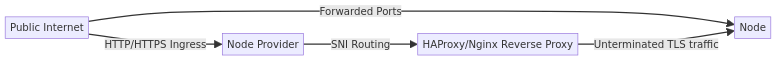
\includegraphics[width=\textwidth]{figures/impl-networking.png}
    \caption{Networking Diagram. Note that blockchain (and the consensus protocol) are not on the data path, so the node performance isn't limited by the consensus speed. Blockchain is on the control path only and is primarily used for tracking reputation.}
    \label{fig:networking_diagram}
\end{figure*}


\subsubsection{Security}

While premium security is a necessity, it often comes with a cost. Techniques such as homomorphic encryption, although secure, can significantly slow down operations and inflate data size by a factor of 10 to 100 or more.

Technologies like Intel SGX and TDX, AMD SEV-SNP, ARM TrustZone, and open-source efforts like UC Berkeley's Keystone offer robust security at a relatively low cost. However, the use of Confidential Computing VMs can lead to a slight performance loss and added complexity. Certain operations are currently unsupported with Confidential Computing VMs:

\begin{enumerate}
    \item Nested virtualization: Running a VM within another VM is not feasible.
    \item Memory overcommitment: Confidential VMs' encrypted memory limits the ability to share or swap out memory, hindering memory overcommitment.
    \item VM snapshots, cloning, and live migration: The hardware-specific encryption keys make it impossible to migrate the encrypted memory state to another host, increasing downtime risk.
    \item Debugging and Inspection: The VM's encrypted and isolated memory state complicates troubleshooting and monitoring.
    \item High-performance Computing (HPC): Direct, low-latency access to hardware resources required by some HPC workloads can be complicated by the additional encryption and isolation layer.
    \item Hardware Compatibility: Not all hardware platforms or devices are compatible with confidential computing technologies.
\end{enumerate}

Despite these challenges, Confidential Computing VMs are invaluable in scenarios where sensitive data needs to be processed or stored securely. These include:

\begin{enumerate}
    \item Private Token Management and Rotation: Confidential computing securely handles sensitive operations like token management and rotation.
    \item SSL Certificate Renewal and Key Storage: Renewing SSL certificates and storing private keys can be securely managed within a confidential computing environment.
    \item Secure Multi-party Computation: Confidential computing provides a secure environment for computation in scenarios where multiple parties need to collaborate on sensitive data.
    \item Data Privacy and Compliance: Confidential computing can help meet strict data privacy and compliance requirements in industries handling sensitive data.
    \item Intellectual Property Protection: Confidential computing ensures that sensitive intellectual property, such as proprietary algorithms or models, are not exposed.
\end{enumerate}

The proposed strategy is to facilitate the use of both regular and Confidential Computing VMs, thereby providing developers with the flexibility to select VM types based on their specific requirements. For example, developers could manage confidential workloads using Confidential Computing VMs, while employing regular VMs for all other workloads. This approach promotes a tailored and efficient use of resources, aligning with the individual needs of each workload.

\subsection{Reputation System}
\label{sec:reputation_system}

The reputation system is the cornerstone of our platform, maintaining simplicity comparable to existing cloud platforms while reliably running conventional workloads on a globally distributed network of node providers. It enhances security, transparency, and fairness in resource allocation. All participants' reputations, including developers and node providers, are tracked via smart contracts on a blockchain.

When a developer pays a node provider, the system charges the node provider a 2\% fee. A portion of this fee is automatically transferred to a DAO-controlled wallet that finances research and development efforts. In return, the reputations of both the developer and the node provider increase by 1\%.

Assuming mostly honest behavior, the reputations of developers and node providers will gradually grow, proportional to the service payment amounts and transactions performed on the platform. All reputations are publicly visible, allowing, but not forcing, node providers and developers to restrict their interactions to high-reputation parties. Additionally, node providers' reputations are used to reward them for offering nodes for rent, making it crucial for all node providers to maintain a high reputation.

If either a node provider or a developer is dissatisfied with the service or collaboration, they can spend their reputation to reduce the other's reputation. The sender's reputation decreases by the amount spent, while the receiver's reputation decreases by a higher amount, such as 200\%, to incentivize honest and cooperative behavior. For members with high reputations, these reductions can be severe in extreme cases. Spending hard-earned reputation to reduce another party's reputation is not undertaken lightly, as rebuilding reputation takes significant time and money.

Reputation is hard to earn and easy to lose, encouraging all parties to uphold high standards of quality, communication, and integrity at all times, while still offering a means to penalize potentially dishonest or malicious behavior, in a general and transparent manner.

\begin{figure}[ht]
    \centering
    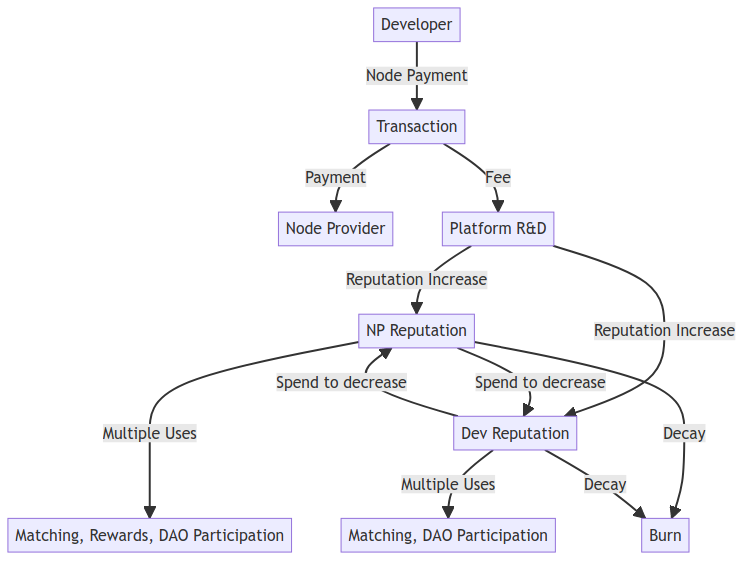
\includegraphics[width=\columnwidth]{figures/impl-reputation.png}
    \caption{Reputation tracking system, running on Blockchain.}
    \label{fig:reputation-system}
\end{figure}


\subsection{Resource Allocation}
\label{sec:resource_allocation}

The platform employs a matching engine and, if necessary, machine learning algorithms to efficiently allocate resources and match developers with suitable nodes.

A developer specifies their requirements, which may include some or all of the following:
\begin{itemize}
    \item Acceptable price
    \item Required virtual CPU (vCPU)
    \item Required Random Access Memory (RAM)
    \item Required storage (which can be unlimited)
    \item Required network bandwidth (which can be unlimited)
    \item Minimum node provider reputation
    \item Contract period
\end{itemize}

The matching engine processes these requirements and returns a list of suitable nodes. The developer then selects one or more nodes from this list and sends a request to start the contract. Upon receiving payment from the developer, the matching engine provides a rental contract ID. The developer can use this contract ID to start utilizing the node.

If the developer wishes to extend the rental period, they can make another request at a later time. The process for extending the contract duration is similar to the original rental process, with the key difference being that the developer already has access to the node.


\subsection{Token Economics (Tokenomics)}
\label{sec:token_economics}

The platform tokenomics balances two key components: (1) the Decentralized Cloud Token (DCT), with which all key platform operations are paid, and (2) the actor reputation, which is hard to earn and easy to lose. The reputation is discussed in more details in Section~\ref{sec:reputation_system}.

{\bf Token Minting (Generation) and Distribution.}
Similar to Bitcoin, DC tokens are minted in each new block, occurring approximately every 10 minutes. The initial block mints 50 tokens, and after that the minted tokens are halving every 210,000 blocks. This model is designed to sustain token supply growth at a decreasing rate, with a final cap due to the smallest unit set by the DC token's nine decimal places, calculated to total of approximately 21,000,000 DC tokens.

The distribution of DC tokens received in a block are weighted by their reputation within the protocol. This reputation is dynamically adjusted based on participants' transaction activities and behaviors. The reward distribution uses a square root scaling function to calculate weights, providing diminishing returns on increased reputation scores, thereby maintaining incentives for both high and low-reputation participants.

Importantly, there will be no other DCT generation other than through this minting and rewarding process. There will be no additional token sale, airdrop, or any other form of token distribution. This approach promotes fair distribution of DCT across participants and balances supply and demand over time.

{\bf Project Funding.}
Participation in the DC token reward distribution requires a fee, set at 1/100th of the block reward, creating a steady funding stream for project-related activities. These fees are directed to predetermined wallets, which include known wallets designated for project development. This ensures transparency in funding flows and supports ongoing development efforts.

{\bf Stability, Governance, and Community Engagement.}
The stability and security of the token value are ensured through several mechanisms. Firstly, the supply of DCT is both limited and predictable, which, when balanced against the inherent demand created by developers needing to rent nodes, aids in maintaining market equilibrium. Secondly, the platform's Decentralized Autonomous Organization (DAO) has the capability to implement necessary adjustments to the reward system. This flexibility allows for the mitigation of extreme price volatility. Finally, the platform is committed to adhering to all relevant legal and regulatory standards, further ensuring the security of transactions and the integrity of the token system.

This model would facilitate community input through a transparent proposal system where community members can submit and vote on changes. It will also be possible to implement a delegated governance model, to address potential voter apathy and ensure informed decision-making.

{\bf Token Demand and Supply.}
Developers and node providers need to obtain DCT in order to pay for the registration fee. The DCT token can be obtained on an exchange, and the exchange obtains the token from one of the existing token holders. This creates an inherent demand for DCT. Node providers, on the other hand, will need to cover costs such as electricity and internet connectivity, which may necessitate selling a portion of their DCT. However, some providers may choose to retain a portion of their DCT in anticipation of a price increase, which could, in turn, increase the likelihood of such a price increase and creating a virtuous circle.

{\bf Smart Contract Interoperability.}
The system would run on the Internet Computer platform and DCT would adhere to the ICRC-1 and potentially also newer token standard to ensure compatibility and ease of integration with wallets and exchanges. In the future, an exploration of cross-chain functionality will take place, to enhance liquidity and utility across different blockchain ecosystems.

\subsection{Application Support}
\label{sec:application_support}

The ability to support a wide range of applications is a critical factor for the success of any computing platform. This versatility not only broadens the platform's potential user base but also increases its utility and value for each user. By accommodating various types of applications, from scientific computing and machine learning to web hosting and data storage, the platform can cater to diverse needs and use cases, thereby attracting a wider audience and fostering a vibrant and diverse user community \cite{gawer2002platform}.

Our platform is designed with this versatility in mind. It provides comprehensive support for a wide range of applications, enabling developers to leverage the platform's resources and capabilities to build and deploy various types of applications. This is in line with the best practices in platform design, which emphasize the importance of flexibility and extensibility in supporting diverse applications \cite{meyer1997power}.

To facilitate application development and deployment, the platform provides Application Programming Interfaces (APIs) and Software Development Kits (SDKs). These tools simplify the process for developers to interact with the platform, abstracting away the complexities of the underlying infrastructure. This aligns with the principles of developer experience, which highlight the importance of providing developers with effective tools and resources to enhance their productivity and satisfaction \cite{ko2006exploratory}.

Moreover, the platform is designed to be permissionless, meaning that the community of node providers and developers themselves can decide what kind of support should be added. For instance, there is nothing stopping node providers from adding nodes with GPU support, even though this is not something that is explicitly supported or required by the platform. This permissionless nature fosters innovation and allows the platform to adapt to the evolving needs of its community.

In conclusion, by providing comprehensive application support, continuously adapting to the evolving needs of developers, and allowing the community to drive innovation and expansion, our platform aims to be a versatile and valuable tool for a wide range of applications.

\section{Benefits and Impact}
\label{sec:benefits_and_impact}

The proposed decentralized cloud platform offers numerous potential benefits and could significantly impact the cloud computing industry:

\begin{itemize}
    \item \textbf{Democratization of Resources:} By leveraging unused computational resources globally, the platform democratizes access to cloud computing. This could make cloud services more affordable and accessible, particularly in developing countries or remote areas.

    \textit{Quantitative Projection:} We estimate that this democratization could potentially reduce entry-level cloud computing costs by 30-50\% compared to current centralized providers.

    \item \textbf{Cost Reduction:} The platform could significantly reduce cloud computing costs by eliminating the need for expensive data centers and using more efficient resource allocation.

    \textit{Quantitative Projection:} Based on our models, enterprises could see a 20-40\% reduction in their cloud computing expenses, potentially saving millions for large-scale operations.

    \item \textbf{Increased Competition:} By providing a decentralized alternative to traditional cloud providers, the platform promotes competition in the cloud computing market. This could drive down prices compared to conventional cloud providers and spur innovation.

    \textit{Quantitative Estimate:} We project a 15-25\% increase in the number of viable cloud service providers within the first three years of platform adoption.

    \item \textbf{Environmental Sustainability:} Using existing computational resources more efficiently could reduce the need for new data centers, contributing to environmental sustainability.

    \textit{Quantitative Projection:} We estimate that widespread adoption of our platform could reduce the carbon footprint associated with cloud computing by 10-20\% over five years.

    \item \textbf{Resilience and Security:} The decentralized nature of the platform enhances resilience against attacks and failures. The use of blockchain technology and our reputation system further bolsters security and transparency.

    \textit{Quantitative Estimate:} We project a 40-60\% reduction in the impact of individual node failures or security breaches compared to centralized systems.
\end{itemize}

The impact of the platform could extend far beyond the cloud computing industry. By making cloud computing more affordable and accessible, it could enable new applications and services across various sectors:

\begin{itemize}
    \item \textbf{Scientific Research:} Affordable access to high-performance computing could accelerate research in fields like genomics, climate modeling, and particle physics.

    \textit{Case Study:} A small university research team could leverage the platform to run complex climate models at 1/3 the cost of traditional cloud services, enabling more comprehensive studies on a limited budget.

    \item \textbf{Education:} Educational institutions could provide better computational resources to students, enhancing learning experiences in computer science, data analysis, and other tech-intensive fields.

    \textit{Scenario:} A rural high school could set up a advanced computing lab using our platform, giving students access to resources previously available only in well-funded urban schools.

    \item \textbf{Healthcare:} Improved access to computational resources could enhance medical imaging analysis, drug discovery processes, and personalized medicine initiatives.

    \textit{Case Study:} A startup developing AI for early cancer detection could use our platform to process millions of medical images at 50\% lower cost, potentially bringing their life-saving technology to market faster.

    \item \textbf{Small Business and Startups:} Reduced costs and easier access to cloud resources could lower barriers to entry for tech startups and enable small businesses to leverage advanced analytics and AI.

    \textit{Scenario:} A local retail chain could implement sophisticated inventory management and customer behavior analysis, previously only feasible for large corporations, improving their competitiveness.
\end{itemize}

In summary, our decentralized cloud platform has the potential to democratize access to advanced computing resources, foster innovation across multiple sectors, and contribute to a more sustainable and equitable digital economy. The projected cost savings, improved accessibility, and enhanced performance could catalyze breakthroughs in science, education, healthcare, and business, driving societal progress and economic growth.

\section{Conclusion}
\label{sec:conclusion}

In conclusion, the proposed decentralized cloud platform signifies a substantial advancement in the field of cloud computing. By harnessing the capabilities of distributed systems and blockchain technology, this platform is poised to democratize access to computational resources, reduce costs, stimulate competition, enhance environmental sustainability, and improve resilience and security.

Certainly, the implementation of such a transformative platform will present its own set of challenges. However, the potential benefits and the profound impact of this platform make it a venture of great significance. We are not merely suggesting a minor modification to the cloud computing industry - we are advocating for a comprehensive transformation with far-reaching implications for society and the economy.

Contrary to the majority of preceding web3 projects, our platform does not necessitate a complete overhaul of existing applications. These applications can continue to operate as usual, but on a decentralized cloud. A cloud that does not tolerate misconduct from cloud service providers, and does not succumb to vendor lock-in. Cloud that we all deserve. Cloud as it should have been.


% \backmatter

\printbibliography

% \appendix
% \input{appendix}

\end{document}
